\section{Visualisation des données}
Une page de visualisation des données a été crée en utilisaant les langanges HTML, CSS, PHP, JavaScript et une librairie permettant la création de graphique. Sur cette page on retrouve par exemple tous les informations concernant un noeud, tous les informations sur les capteurs d'un noeud données ainsi que les données des capteurs localisés sur un noeud données représentés sous forme de graphiques comme dans comme dans la figure.
Une des amélioration a apporté à la visualisation, serait de pouvoir croiser les données pour pourvoir permettre une comparaison rapide des relevés capteurs. En effet, pour l'instant, pour une même données \begin{math}x \end{math} (exemple : température de l'aire) mesurée par deux capteurs distincts \begin{math}C_{1}\end{math} et \begin{math}C_{2}\end{math}, on a deux graphiques distincts, ces derniers étant construit par capteurs. Le but serait donc de combiner les 2 graphiques en un seul graphique ce qui permettrait une comparaison plus rapide
\begin{figure}
    \centering
    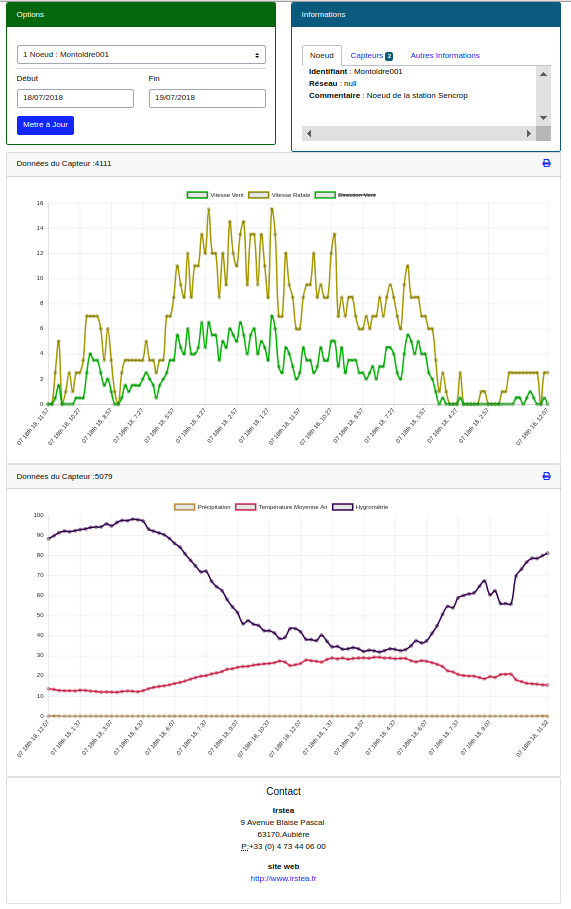
\includegraphics[height=1\textheight]{images/db_visualisation.png}
    \caption{page de visualisation des données}
    \label{fig:page de visualisation des données}
\end{figure}


